%╔════════════════════════════╗
%║	  Szablon dostosował	  ║
%║	mgr inż. Dawid Kotlarski  ║
%║		  06.10.2024		  ║
%╚════════════════════════════╝
\documentclass[12pt,twoside,a4paper,openany]{article}

    % ------------------------------------------------------------------------
% PAKIETY
% ------------------------------------------------------------------------

%różne pakiety matematyczne, warto przejrzeć dokumentację, muszą być powyżej ustawień językowych.
\usepackage{mathrsfs}   %Różne symbole matematyczne opisane w katalogu ~\doc\latex\comprehensive. Zamienia \mathcal{L} ze zwykłego L na L-transformatę.
\usepackage{eucal}      %Różne symbole matematyczne.
\usepackage{amssymb}    %Różne symbole matematyczne.
\usepackage{amsmath}    %Dodatkowe funkcje matematyczne, np. polecenie \dfac{}{} skladajace ulamek w trybie wystawionym (porównaj $\dfrac{1}{2}$, a $\frac{1}{2}$).

%język polski i klawiatura
\usepackage[polish]{babel}
%\usepackage{qtimes} % czcionka Times new Roman
\usepackage[OT4]{polski}
%\usepackage[cp1250]{inputenc}                       %Strona kodowa polskich znaków.

%obsługa pdf'a
\usepackage[pdftex,usenames,dvipsnames]{color}      %Obsługa kolorów. Opcje usenames i dvipsnames wprowadzają dodatkowe nazwy kolorow.
\usepackage[pdftex,pagebackref=false,draft=false,pdfpagelabels=false,colorlinks=true,urlcolor=blue,linkcolor=black,citecolor=green,pdfstartview=FitH,pdfstartpage=1,pdfpagemode=UseOutlines,bookmarks=true,bookmarksopen=true,bookmarksopenlevel=2,bookmarksnumbered=true,pdfauthor={Dawid Kotlarski},pdftitle={Dokumentacja Projektowa},pdfsubject={},pdfkeywords={transient recovery voltage trv},unicode=true]{hyperref}   %Opcja pagebackref=true dotyczy bibliografii: pokazuje w spisie literatury numery stron, na których odwołano się do danej pozycji.

%bibliografia
%\usepackage[numbers,sort&compress]{natbib}  %Porządkuje zawartość odnośników do literatury, np. [2-4,6]. Musi być pod pdf'em, a styl bibliogfafii musi mieć nazwę z dodatkiem 'nat', np. \bibliographystyle{unsrtnat} (w kolejności cytowania).
\usepackage[
	backend=biber,
	style=numeric,
	sorting=none
]{biblatex}
\addbibresource{bibliografia.bib}
\usepackage{hypernat}                       %Potrzebna pakietowi natbib do wspolpracy z pakietem hyperref (wazna kolejnosc: 1. hyperref, 2. natbib, 3. hypernat).

%grafika i geometria strony
\usepackage{extsizes}           %Dostepne inne rozmiary czcionek, np. 14 w poleceniu: \documentclass[14pt]{article}.
\usepackage[final]{graphicx}
\usepackage[a4paper,left=3.5cm,right=2.5cm,top=2.5cm,bottom=2.5cm]{geometry}

%strona tytułowa
\usepackage{strona_tytulowa}

%inne
\usepackage[hide]{todo}                     %Wprowadza polecenie \todo{treść}. Opcje pakietu: hide/show. Polecenie \todos ma byc na koncu dokumentu, wszystkie \todo{} po \todos sa ignorowane.
\usepackage[basic,physics]{circ}            %Wprowadza środowisko circuit do rysowania obwodów elektrycznych. Musi byc poniżej pakietow językowych.
\usepackage[sf,bf,outermarks]{titlesec}     %Troszczy się o wygląd tytułów rozdziałów (section, subsection, ...). sf oznacza czcionkę sans serif (typu arial), bf -- bold. U mnie: oddzielna linia dla naglowku paragraph. Patrz tez: tocloft -- lepiej robi format spisu tresci.
\usepackage{tocloft}                        %Troszczy się o format spisu trsci.
\usepackage{expdlist}    %Zmienia definicję środowiska description, daje większe możliwości wpływu na wygląd listy.
\usepackage{flafter}     %Wprowadza parametr [tb] do polecenia \suppressfloats[t] (polecenie to powoduje nie umieszczanie rysunkow, tabel itp. na stronach, na ktorych jest to polecenie (np. moze byc to stroma z tytulem rozdzialu, ktory chcemy zeby byl u samej gory, a nie np. pod rysunkiem)).
\usepackage{array}       %Ładniej drukuje tabelki (np. daje wiecej miejsca w komorkach -- nie są tak ścieśnione, jak bez tego pakietu).
\usepackage{listings}    %Listingi programow.
\usepackage[format=hang,labelsep=period,labelfont={bf,small},textfont=small]{caption}   %Formatuje podpisy pod rysunkami i tabelami. Parametr 'hang' powoduje wcięcie kolejnych linii podpisu na szerokosc nazwy podpisu, np. 'Rysunek 1.'.
\usepackage{appendix}    %Troszczy się o załączniki.
\usepackage{floatflt}    %Troszczy się o oblewanie rysunkow tekstem.
\usepackage{here}        %Wprowadza dodtkowy parametr umiejscowienia rysunków, tabel, itp.: H (duże). Umiejscawia obiekty ruchome dokladnie tam gdzie są w kodzie źródłowym dokumentu.
\usepackage{makeidx}     %Troszczy się o indeks (skorowidz).

%nieużywane, ale potencjalnie przydatne
\usepackage{sectsty}           %Formatuje nagłówki, np. żeby były kolorowe -- polecenie: \allsectionsfont{\color{Blue}}.
%\usepackage{version}           %Wersje dokumentu.

%============
\usepackage{longtable}			%tabelka
%============

%============
% Ustawienia listingów do kodu
%============

\usepackage{listings}
\usepackage{xcolor}

\definecolor{codegreen}{rgb}{0,0.6,0}
\definecolor{codegray}{rgb}{0.5,0.5,0.5}
\definecolor{codepurple}{rgb}{0.58,0,0.82}
\definecolor{backcolour}{rgb}{0.95,0.95,0.92}

% Definicja stylu "mystyle"
\lstdefinestyle{mystyle}{
	backgroundcolor=\color{backcolour},
	commentstyle=\color{codegreen},
	keywordstyle=\color{blue},	%magenta
	numberstyle=\tiny\color{codegray},
	stringstyle=\color{codepurple},
	basicstyle=\ttfamily\footnotesize,
	breakatwhitespace=false,
	breaklines=true,
	captionpos=b,
	keepspaces=true,
	numbers=left,
	numbersep=5pt,
	showspaces=false,
	showstringspaces=false,
	showtabs=false,
	tabsize=2
}

\lstset{style=mystyle} % Deklaracja aktywnego stylu
%===========

%PAGINA GÓRNA I DOLNA
\usepackage{fancyhdr}          %Dodaje naglowki jakie się chce.
\pagestyle{fancy}
\fancyhf{}
% numery stron w paginie dolnej na srodku
\fancyfoot[C]{\scriptsize DOKUMENTACJA PROJEKTU – ZAAWANSOWANE PROGRAMOWANIE \\
	\normalsize\sffamily  \thepage}


%\fancyhead[L]{\small\sffamily \nouppercase{\leftmark}}
\fancyhead[C]{\footnotesize \textit{AKADEMIA NAUK STOSOWANYCH W NOWYM SĄCZU}\\}

\renewcommand{\headrulewidth}{0.4pt}
\renewcommand{\footrulewidth}{0.4pt}

    % ------------------------------------------------------------------------
% USTAWIENIA
% ------------------------------------------------------------------------

% ------------------------------------------------------------------------
%   Kropki po numerach sekcji, podsekcji, itd.
%   Np. 1.2. Tytuł podrozdziału
% ------------------------------------------------------------------------
\makeatletter
\def\numberline#1{\hb@xt@\@tempdima{#1.\hfil}}                      %kropki w spisie treści
\renewcommand*\@seccntformat[1]{\csname the#1\endcsname.\enspace}   %kropki w treści dokumentu
\makeatother

% ------------------------------------------------------------------------
%   Numeracja równań, rysunków i tabel
%   Np.: (1.2), gdzie:
%   1 - numer sekcji, 2 - numer równania, rysunku, tabeli
%   Uwaga ogólna: o otoczeniu figure ma być najpierw \caption{}, potem \label{}, inaczej odnośnik nie działa!
% ------------------------------------------------------------------------
\makeatletter
\@addtoreset{equation}{section} %resetuje licznik po rozpoczęciu nowej sekcji
\renewcommand{\theequation}{{\thesection}.\@arabic\c@equation} %dodaje kropki

\@addtoreset{figure}{section}
\renewcommand{\thefigure}{{\thesection}.\@arabic\c@figure}

\@addtoreset{table}{section}
\renewcommand{\thetable}{{\thesection}.\@arabic\c@table}
\makeatother

% ------------------------------------------------------------------------
% Tablica
% ------------------------------------------------------------------------
\newenvironment{tabela}[3]
{
    \begin{table}[!htb]
        \centering
        \caption[#1]{#2}
        \vskip 9pt
        #3
        }{
    \end{table}
}

% ------------------------------------------------------------------------
% Dostosowanie wyglądu pozycji listy \todos, np. zamiast 'p.' jest 'str.'
% ------------------------------------------------------------------------
\renewcommand{\todoitem}[2]{%
    \item \label{todo:\thetodo}%
    \ifx#1\todomark%
    \else\textbf{#1 }%
    \fi%
    (str.~\pageref{todopage:\thetodo})\ #2}
\renewcommand{\todoname}{Do zrobienia\ldots}
\renewcommand{\todomark}{~uzupełnić}

% ------------------------------------------------------------------------
% Definicje
% ------------------------------------------------------------------------
\def\nonumsection#1{%
    \section*{#1}%
    \addcontentsline{toc}{section}{#1}%
}
\def\nonumsubsection#1{%
    \subsection*{#1}%
    \addcontentsline{toc}{subsection}{#1}%
}
\reversemarginpar %umieszcza notki po lewej stronie, czyli tam gdzie jest więcej miejsca
\def\notka#1{%
    \marginpar{\footnotesize{#1}}%
}
\def\mathcal#1{%
    \mathscr{#1}%
}
\newcommand{\atp}{ATP/EMTP} % Inaczej: \def\atp{ATP/EMTP}

% ------------------------------------------------------------------------
% Inne
% ------------------------------------------------------------------------
\frenchspacing
\hyphenation{ATP/-EMTP}             %dzielenie wyrazu w danym miejscu
\setlength{\parskip}{3pt}           %odstęp pomiędzy akapitami
\linespread{1.3}                    %odstęp pomiędzy liniami (interlinia)
\setcounter{tocdepth}{4}            %uwzględnianie w spisie treści czterech poziomów sekcji
\setcounter{secnumdepth}{4}         %numerowanie do czwartego poziomu sekcji 
\titleformat{\paragraph}[hang]      %wygląd nagłówków
{\normalfont\sffamily\bfseries}{\theparagraph}{1em}{}

% Makro do zdjęć
\newcommand*{\fg}[4][!htb]{
    \begin{figure}[#1]
        \begin{center}
            \includegraphics[width=8cm]{#2}
            \caption{#3}
            \label{#4}
        \end{center}
    \end{figure}
}

\newcommand*{\Oznacz}[2]{\ref{#1:#2} (s.~\pageref{#1:#2})
}

\newcommand*{\OznaczZdjecie}[1]{
    Rysunek \Oznacz{rys}{#1}
}

\newcommand*{\OznaczKod}[1]{
    \Oznacz{lst}{#1}
}


    %polecenia zdefiniowane w pakiecie strona_tytulowa.sty
    \title{ProjectName}		%...Wpisać nazwę projektu...
    \author{AuthorName}
    \authorI{}
    \authorII{}		%jeśli są dwie osoby w projekcie to zostawiamy:    \authorII{}
		
	\uczelnia{AKADEMIA NAUK STOSOWANYCH \\W NOWYM SĄCZU}
    \instytut{Wydział Nauk Inżynieryjnych}
    \kierunek{Katedra Informatyki}
    \praca{DOKUMENTACJA PROJEKTOWA}
    \przedmiot{ZAAWANSOWANE PROGRAMOWANIE}
    \prowadzacy{mgr inż. Dawid Kotlarski}
    \rok{2024}


%definicja składni mikrotik
\usepackage{fancyvrb}
\DefineVerbatimEnvironment{MT}{Verbatim}%
{commandchars=\+\[\],fontsize=\small,formatcom=\color{red},frame=lines,baselinestretch=1,} 
\let\mt\verb 
%zakonczenie definicji składni mikrotik

\usepackage{fancyhdr}    %biblioteka do nagłówka i stopki

			
\begin{document}

\renewcommand{\figurename}{Rys.}    %musi byc pod \begin{document}, bo w~tym miejscu pakiet 'babel' narzuca swoje ustawienia
\renewcommand{\tablename}{Tab.}     %j.w.
\thispagestyle{empty}               %na tej stronie: brak numeru
\stronatytulowa                     %strona tytułowa tworzona przez pakiet strona_tytulowa.tex

\pagestyle{fancy}

\newpage

%formatowanie spisu treści i~nagłówków
\renewcommand{\cftbeforesecskip}{8pt}
\renewcommand{\cftsecafterpnum}{\vskip 8pt}
\renewcommand{\cftparskip}{3pt}
\renewcommand{\cfttoctitlefont}{\Large\bfseries\sffamily}
\renewcommand{\cftsecfont}{\bfseries\sffamily}
\renewcommand{\cftsubsecfont}{\sffamily}
\renewcommand{\cftsubsubsecfont}{\sffamily}
\renewcommand{\cftparafont}{\sffamily}
%koniec formatowania spisu treści i nagłówków

\tableofcontents    %spis treści
\thispagestyle{fancy}
\newpage


\newpage


%%%%%%%%%%%%%%%%%%% treść główna dokumentu %%%%%%%%%%%%%%%%%%%%%%%%%

\newpage
\section{Ogólne określenie wymagań}		%1
%Określenie celu pracy, co chcemy uzyskać, jakie przewidujemy wyniki

\hspace{0.60cm}Tutaj może coś być wpisane.

\subsection{Przykład}  %1.1       

\hspace{0.60cm}Tak zaczynamy pisanie pierwszego akapitu. Jeśli chcemy napisać przypis do bibliografii wykonujemy to w~ten sposób\footnote{Przykład odnośnika do książki\cite{legierski}.}.

%rysunek
\begin{figure}[!htb]
  \begin{center}
    
\includegraphics[width=8cm]{rys/ans.png}
    \caption{Logo}
    \label{rys:rysunek001}
  \end{center}
\end{figure}

\fg{rys/ans.png}{Logo}{rys:rysunek003}

Tutaj może coś być wpisane. \\Tutaj może coś być wpisane\footnote{Przykład odnośnika do strony www\cite{www1}.}.
Rysunek \ref{rys:rysunek001} (s. \pageref{rys:rysunek001}) pokazuje przykładową ilustrację.

%tabelka
\begin{tabela}
  %uwaga: w nawiasach [] nie może być odnośnika do literatury, jeżeli w dokumencie jest spis rysunków na początku, a spis literatury jest w kolejności cytowania (zmienia to numeracji)
  {Tabelka przykładowa}	%opis w spisie tabel
  {Tabelka przykładowa}	%opis przy tabeli
  {
    \begin{tabular}{|c|c|} \hline
      $U_n$ & $I_{zw}$ \\ \hline
      $kV$  & $\%$     \\ \hline
      7.2   & 100      \\ \hline
    \end{tabular}
  }
  \label{tab:tablica001}
\end{tabela}

% Kod

Listing kodu

\begin{lstlisting}[caption=Przykładowy kod 001, label={lst:listing-cpp}, language=C++]
#include <iostream>
#include <cstdlib>
#include <ctime>
using namespace std;

/*
liczby pseldolosowe
*/

int main(int argc, char** argv) {
	
	int tab[10][10];
	
	for(int i=0;i<10;i++)
	for(int j=0;j<10;j++)
	tab[i][j]=0;
	
	srand(time(NULL));		//generowanie z czasu
	int min=3;
	int max=7;
	for(int i=0;i<10;i++)
	for(int j=0;j<10;j++)		
	tab[i][j]=(rand()%(max-min+1))+min;	
	
	for(int i=0;i<10;i++)
	{
		for(int j=0;j<10;j++)
		cout<<tab[i][j]<<" ";	
		cout<<endl;
	}
	
	return 0;
}
\end{lstlisting}

Tutaj może coś być wpisane. Tutaj może coś być wpisane. Tutaj może coś być wpisane. Tabela \ref{tab:tablica001} (s. \pageref{tab:tablica001}) pokazuje sposoby użycia trybu matematycznego.

Kod \ref{lst:listing-cpp} (s. \pageref{lst:listing-cpp}) przedstawia sposób generowania liczb pseudolosowych. Kod \ref{lst:listing-cpp2} (s. \pageref{lst:listing-cpp2}) przedstawia generowanie pliku HTML.

Alternatywna metoda wklejenia kodu:

\lstinputlisting[caption=Przykładowy kod 002, label={lst:listing-cpp2}, language=C++]{kod/main.cpp}


\subsection{Instalacja}  %1.2

\hspace{0.60cm}Poniżej są opisane kroki potrzebne do instalacji \LaTeX 'a oraz do używania tego szablonu.

Na początku instalujemy \TeX{}Live\footnote{Instalka na stronie  https://www.tug.org/texlive/acquire-netinstall.html\cite{www2}.}. Ściągamy plik instalacyjny, zajmuje około 25MB. Podczas instalacji można wybrać do zainstalowania różne kolekcje pakietów. Jeśli nie ma problemów z miejscem na dysku to można zainstalować wszystkie, wtedy nie będzie problemu z brakującymi pakietami i błędami. Po wybraniu kolekcji brakujące pliki są pobierane z internetu. Pełna instalacja programu zajmuje około 8GB. Najlepiej zostawić instalację na noc, ponieważ proces zabiera sporo czasu. Warto ustawić komputer tak, aby się nie wyłączył lub nie uśpił. Warto także przed instalacją zablokować antywirusa, ponieważ może blokować niektóre z komponentów.

Następnie instalujemy \TeX{}studio\footnote{Plik instalacyjny na stronie  https://www.texstudio.org\cite{www3}.}. Ściągamy plik instalacyjny zajmujący około 120MB. Instalacja przebiega standardowo.

%rysunek
\begin{figure}[!hbt]
  \begin{center}
    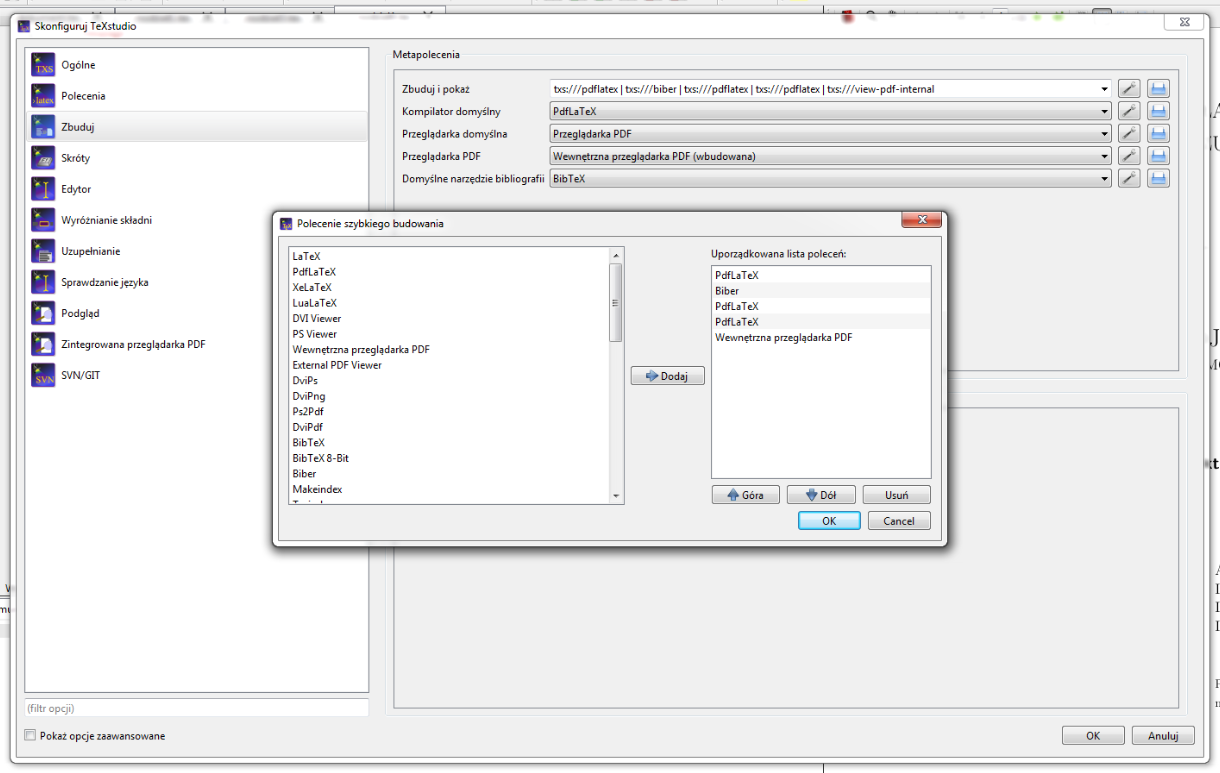
\includegraphics[width=\linewidth]{rys/ustawienie.png}
    \caption{Ustawienie TeXstudio}
    \label{rys:ustawienia}
  \end{center}
\end{figure}

Następnym krokiem jest ustawienie w \TeX{}Studio kolejności budowania projektu. Należy wybrać zakładkę: ,,Opcje/Konfiguruj \TeX{}studio...''. W otwartym oknie przechodzimy na zakładkę ,,Zbuduj''. Na rysunku \ref{rys:ustawienia} (s. \pageref{rys:ustawienia}) pokazany jest zrzut ekranu z konfiguracją. W linijce ,,Zbuduj i pokaż'' klikamy ikonę klucza, żeby przejść do konfiguracji polecenia. W otwartym oknie ustawić kolejność tak jak pokazano na rysunku.


\newpage
\section{Analiza problemu}		%2
%Napisać gdzie używa się tego algorytmu
%Opisać sposób działania programu/algorytmu
%Napisać spsoób wykorzystania algorytmu po przez wykonanie przykładu (np. mnożenie macierzy - wykonać ręcznie przykład z mnożeniem macierzy pokazujący jak mnoży się macierz ręcznie)
%Jeśli zadanie zakłada przedstawienie jakiegoś narzędzia (np. git, AI) należy opisać narzędzie
Analizowany problem dotyczy przetwarzania, organizacji i analizy danych energetycznych zapisanych w formacie CSV. Dane te zawierają kluczowe informacje dotyczące autokonsumpcji, eksportu, importu, poboru oraz produkcji energii w wybranych przedziałach czasowych. Celem projektu jest stworzenie wszechstronnej aplikacji, która umożliwi efektywne zarządzanie danymi, organizując je w sposób hierarchiczny, a także zapewni użytkownikowi narzędzia do ich analizy i raportowania.
\\
W centrum problemu leży potrzeba radzenia sobie z dużymi zbiorami danych o różnorodnej jakości i strukturze. Program ma być odporny na typowe problemy związane z nieprzewidywalnością danych wejściowych, takie jak brak ciągłości czasowej, powtarzające się rekordy, puste linie czy brakujące wartości. Dodatkowo, projekt wymaga implementacji struktur danych, które umożliwią szybkie i elastyczne przetwarzanie danych w wybranych przedziałach czasowych, zgodnie z założeniami organizacji w hierarchiczne drzewo.
\subsection{Parsowanie i przygotowanie danych}
Prasowanie danych (ang. data wrangling) jest kluczowym etapem w procesie przygotowania danych do analizy, szczególnie w przypadku dużych zbiorów danych, takich jak te, które są przechowywane w formacie CSV. W kontekście tego projektu, parsowanie danych obejmuje szereg czynności mających na celu oczyszczenie, przekształcenie i zorganizowanie surowych danych energetycznych w sposób umożliwiający ich efektywne przetwarzanie oraz analizę. Dla tego projektu kluczowe aspekty prasowania danych to:
\begin{itemize}
    \item \textbf{Obsługa brakujących danych} - Pliki CSV mogą zawierać rekordy, w których brakują niektóre wartości, np. dane o autokonsumpcji, eksporcie czy produkcji energii. W takich przypadkach konieczne jest wdrożenie metod ich obsługi, takich jak usuwanie wierszy z brakującymi danymi lub ich uzupełnianie na podstawie dostępnych informacji, np. przy użyciu interpolacji.
    \item \textbf{Eliminowanie duplikatów} - W procesie wczytywania danych mogą występować powtarzające się wiersze, które prowadzą do błędnych obliczeń lub zafałszowanej analizy. Dlatego ważne jest, by aplikacja automatycznie identyfikowała i usuwała duplikaty z pliku CSV, aby zapewnić spójność i dokładność danych.
    \newpage
    \item \textbf{Walidacja danych} - Wiele plików CSV zawiera dane, które mogą być zapisane w nieodpowiednim formacie lub zawierać błędne informacje, np. błędne daty, godziny spoza dozwolonych przedziałów czy wartości liczbowe w złym formacie. Program musi sprawdzać poprawność danych i odrzucać te, które nie spełniają wymagań określonych w specyfikacji. Przykładem może być sprawdzenie, czy godziny pomiaru są w poprawnym formacie 24-godzinnym lub upewnienie się, że wartości dotyczące autokonsumpcji nie są ujemne.
    \item \textbf{Logowanie i raportowanie błędów} - Ważnym elementem prasowania danych jest także tworzenie raportów o błędach, które umożliwiają analizę nieprawidłowości w plikach CSV. Przykładowo, system powinien zapisywać informacje o odrzuconych rekordach, wskazując przyczyny ich odrzucenia (np. brakujące dane, błędne formaty). Taki raport może być pomocny zarówno w diagnostyce problemów, jak i w przyszłym doskonaleniu procesu przetwarzania danych.
\end{itemize}
Parsowanie danych jest więc kluczowym etapem w całym procesie analizy, który umożliwia dalsze, zaawansowane operacje na danych. Dzięki odpowiedniemu oczyszczeniu i organizacji danych, aplikacja będzie w stanie działać szybko, precyzyjnie i bezbłędnie, oferując użytkownikowi wysoką jakość wyników analizy.
\subsection{Sposób na rozwiązanie problemu}
W celu rozwiązania problemu przyjęto następujące założenia:
\\ \\
\textbf{Format danych wejściowych}
\\
Dane w pliku CSV składają się z kolumn:
\begin{itemize}
    \item Data i godzina pomiaru,
    \item Autokonsumpcja (energia zużywana na bieżąco),
    \item Eksport (energia wysyłana do sieci),
    \item Import (energia pobierana z sieci),
    \item Pobór (całkowita energia zużyta),
    \item Produkcja (energia wytworzona przez falownik).
\end{itemize}
\newpage
\noindent \textbf{Struktura organizacji danych}
\\
Dane mają być przechowywane w strukturze drzewa, której poziomy odpowiadają kolejno:
\begin{itemize}
    \item Rokowi,
    \item Miesiącowi,
    \item Dniowi,
    \item Ćwiartkom dnia (00:00–5:45, 6:00–11:45, 12:00–17:45, 18:00–23:45).
\end{itemize}
Drzewo powinno umożliwiać dostęp do danych w dowolnym przedziale czasowym.
\\ \\
\textbf{Obłsuga danych wejściowych}
\\
Program musi obsługiwać dane o nieprzewidywalnej strukturze, w tym:
\begin{itemize}
    \item Puste linie,
    \item Niekompletne rekordy,
    \item Powtarzające się wiersze.
\end{itemize}
Wszystkie błędne dane powinny być odrzucane, a ich analiza powinna być logowana w dwóch plikach: jeden dla pełnego raportu procesu, a drugi dla szczegółowego opisu błędów.
\\ \\
\textbf{Funkcjonalność aplikacji}
\\ 
Program ma oferować użytkownikowi możliwość interakcji za pomocą menu, które obejmuje:
\begin{itemize}
    \item Wczytywanie danych z pliku CSV,
    \item Zapisywanie i odczytywanie danych w formacie binarnym,
    \item Analizę danych, w tym obliczanie sum, średnich i porównania wartości w różnych przedziałach czasowych,
    \item Filtrowanie rekordów na podstawie określonych kryteriów.
\end{itemize}
\newpage
\subsection{Ograniczenia i wyzwania}
W trakcie analizy zidentyfikowano potencjalne ograniczenia i trudności:
\\ \\
\textbf{Wydajność:}
\begin{itemize}
    \item Przetwarzanie dużych plików CSV może wymagać znacznych zasobów pamięci i mocy obliczeniowej.
    \item Konieczne jest zaimplementowanie wydajnych algorytmów oraz odpowiedniego zarządzania pamięcią, aby uniknąć spowolnień.
\end{itemize}
\textbf{Nieprzewidywalność danych:}
\begin{itemize}
    \item Dane mogą być niekompletne, powtarzające się lub zapisane w różnej kolejności, co wymaga dokładnej walidacji i przetwarzania.
\end{itemize}
\textbf{Złożoność struktury drzewa:}
\begin{itemize}
    \item Implementacja drzewa z wieloma poziomami wymaga precyzyjnego projektowania, szczególnie w przypadku braku ciągłości czasowej w danych.
\end{itemize}
\textbf{Synchronizacja modułów:}
\begin{itemize}
    \item Zapewnienie, że różne moduły programu (wczytywanie danych, operacje na drzewie, zapisywanie do plików) działają spójnie, może być wyzwaniem.
\end{itemize}
\textbf{Obsługa błędów:}
\begin{itemize}
    \item Program musi być odporny na awarie wynikające z nieprawidłowych danych, jednocześnie generując szczegółowe raporty o błędach.
\end{itemize}
\newpage
\subsection{Wykorzystanie aplikacji w praktyce}
\textbf{Zarządzanie energią w budynkach komercyjnych i mieszkalnych}: \\
Aplikacja może być wykorzystana w inteligentnych budynkach (tzw. smart buildings) do monitorowania i optymalizacji zużycia energii.
\begin{itemize}
    \item Monitorowanie autokonsumpcji - Analiza, ile energii zużywa budynek w czasie rzeczywistym, np. dla budynków wyposażonych w panele fotowoltaiczne.
    \item Optymalizacja zużycia - Identyfikacja okresów szczytowego poboru energii, co pozwala na dostosowanie harmonogramu pracy urządzeń elektrycznych.
    \item Raportowanie kosztów - Generowanie raportów zużycia i oszczędności, co pomaga użytkownikom indywidualnym i przedsiębiorstwom kontrolować koszty energii.
\end{itemize}
\textbf{Zarządzanie farmami fotowoltaicznymi i wiatrowymi}: \\
Farmy produkujące energię odnawialną wymagają precyzyjnych narzędzi do monitorowania i analizy danych.
\begin{itemize}
    \item Monitorowanie wydajności paneli fotowoltaicznych - Aplikacja może pomóc w analizie, jak skutecznie działają panele w różnych warunkach pogodowych.
    \item Zarządzanie eksportem energii do sieci - Umożliwia optymalne zarządzanie przesyłem energii do sieci energetycznej i minimalizację strat.
    \item Identyfikacja usterek - Szybkie wykrywanie problemów, takich jak niesprawne panele czy turbiny, na podstawie analizy odchyłów w danych energetycznych.
\end{itemize}
\textbf{Energetyka i dostawcy energii}: \\
Dostawcy energii mogą wykorzystać aplikację do monitorowania przepływów energii i optymalizacji jej dystrybucji. 
\begin{itemize}
    \item Analiza eksportu i importu energii - Umożliwia ocenę, ile energii jest przesyłane między różnymi punktami sieci, oraz identyfikację miejsc przeciążenia sieci.
    \item Prognozowanie zapotrzebowania na energię - Dzięki analizie historycznych danych dostawcy mogą przewidywać zapotrzebowanie na energię w różnych porach dnia i roku.
\end{itemize}
\newpage
\subsection{Możliwości rozwoju i przyszłe rozszerzenia}
Projekt ma potencjał do dalszego rozwoju i implementacji dodatkowych funkcji w przyszłości, które mogą przyczynić się do jeszcze lepszego zarządzania danymi energetycznymi. Potencjalne kierunki rozwoju obejmują:
\begin{itemize}
\item\textbf{Integracja z systemami IoT} - Możliwość łączenia aplikacji z urządzeniami IoT, takimi jak inteligentne liczniki energii, czujniki czy panele fotowoltaiczne, pozwoli na zbieranie danych w czasie rzeczywistym oraz ich natychmiastową analizę, co umożliwi szybszą reakcję na zmiany w zużyciu energii.
\item\textbf{Predykcja i sztuczna inteligencja} - W przyszłości aplikacja może być rozbudowana o moduł predykcji zapotrzebowania na energię na podstawie analizy dużych zbiorów danych. Sztuczna inteligencja (AI) mogłaby przewidywać wzorce zużycia energii, identyfikować anomalie i proponować optymalizację w czasie rzeczywistym.
\item\textbf{Zwiększenie wydajności algorytmów przetwarzania danych} - Ze względu na rosnącą ilość danych energetycznych, możliwe jest zaimplementowanie algorytmów opartych na technologiach rozproszonego przetwarzania, takich jak obliczenia w chmurze, co pozwoli na skalowanie aplikacji do obsługi jeszcze większych zbiorów danych.
\item\textbf{Rozszerzenie formatu wejściowego} - Rozważenie dodania obsługi innych formatów danych wejściowych (np. JSON, XML), co pozwoli na szersze wykorzystanie aplikacji w różnych środowiskach i z różnymi źródłami danych.
\end{itemize}

\newpage
\section{Projektowanie}		%3
%Napisać z jakich narzędzi będziemy korzystać (kompilator, język programowania), git, biblioteki dodatkowe, itp.
%Opisać szczegółowe ustawienia kompilatora (jeśli są), powiązania z bibliotekami, itp.
%Narysować graf, UML, diagram klas, schemat działania algorytmu
%Jeśli zadanie zakłada przedstawienie jakiegoś narzędzia (np. git, AI) należy opisać sposób jego używania
\subsection{Język programowania wykorzystany w projekcie}
W projekcie, zgodnie z wymaganiami, zostanie wykorzystany język C++. Język ten jest idealnym wyborem do implementacji złożonych aplikacji przetwarzających duże zbiory danych, takich jak hierarchiczne struktury drzewa przechowujące dane energetyczne. Dzięki możliwości manualnego zarządzania pamięcią, C++ pozwala na efektywne operowanie na danych o dużej objętości, co jest szczególnie istotne w przypadku analizy informacji zawartych w plikach CSV, które mogą obejmować tysiące lub miliony rekordów. C++ oferuje również zaawansowane wsparcie dla programowania obiektowego, co umożliwia stworzenie klas odpowiadających za węzły drzewa, operacje na danych oraz obsługę plików wejściowych i wyjściowych. Dzięki temu kod będzie modularny, przejrzysty i łatwiejszy do rozbudowy w przyszłości.
\subsection{Narzędzia i technologie wykorzystane w projekcie}
W projekcie wykorzystano następujące narzędzia i technologie, które wspierają zarówno rozwój aplikacji, jak i zapewniają jej odpowiednią jakość oraz funkcjonalność:
\begin{itemize}
    \item \textbf{Google Test} - Framework do testowania jednostkowego, który umożliwia automatyczne testowanie poprawności działania aplikacji w różnych scenariuszach. Google Test pozwala na łatwą integrację z systemami Continuous Integration (CI), co zapewnia automatyczne uruchamianie testów na każdym etapie rozwoju projektu. W projekcie służy do weryfikacji poprawności przetwarzania danych oraz testowania funkcji operujących na strukturze drzewa.
    \item \textbf{CMake} - Narzędzie do konfiguracji procesu budowania projektu. CMake generuje odpowiednie pliki konfiguracyjne dla różnych systemów operacyjnych i kompilatorów, co zapewnia elastyczność i łatwość w budowaniu aplikacji na różnych platformach, takich jak Windows i Linux. Dzięki CMake możliwe jest utrzymanie jednej, spójnej konfiguracji procesu budowy, co upraszcza zarządzanie projektem.
    \item \textbf{Ninja} - Lekki system budowania, który współpracuje z CMake i zapewnia szybkie kompilacje. Ninja został wybrany ze względu na mniejsze zużycie zasobów systemowych w porównaniu do tradycyjnych systemów budowania, co znacząco przyspiesza proces kompilacji i umożliwia efektywne zarządzanie czasem w trakcie rozwijania projektu.
    \item \textbf{Doxygen} -  Narzędzie do generowania dokumentacji na podstawie komentarzy w kodzie źródłowym. Doxygen automatycznie tworzy dokumentację w formacie HTML, co pozwala na łatwiejsze zrozumienie struktury i działania kodu. Dokumentacja generowana przez Doxygen jest dostępna na stronie projektu, co umożliwia łatwiejsze przeglądanie i korzystanie z niej przez przyszłych programistów oraz użytkowników.
    \item \textbf{GitHub Actions} - Platforma CI/CD, która umożliwia automatyczne uruchamianie testów, generowanie dokumentacji oraz wdrażanie aplikacji na repozytorium GitHub. GitHub Actions w tym projekcie służy do uruchamiania testów jednostkowych, weryfikacji konwencji commitów, generowania dokumentacji oraz publikacji wersji na GitHub Pages. Dzięki tej platformie cały proces rozwoju aplikacji jest zautomatyzowany, co znacząco zwiększa efektywność i zapewnia jakość kodu.
    \item \textbf{Github Copilot} - to narzędzie oparte na sztucznej inteligencji, które zostało stworzone przez GitHub we współpracy z OpenAI. Jego głównym celem jest wspomaganie programistów w codziennej pracy poprzez automatyczne sugerowanie fragmentów kodu, funkcji czy całych bloków logicznych na podstawie kontekstu i opisów wprowadzonych przez użytkownika. Copilot działa jako rozszerzenie do popularnych edytorów kodu, takich jak Visual Studio Code, i jest w stanie uczyć się na podstawie istniejącego kodu, co pozwala na dostosowywanie sugestii do bieżącego projektu.
\end{itemize}
\subsection{Zarządzanie projektem i współpraca w zespole}
W projekcie szczególną uwagę poświęcono efektywnemu zarządzaniu procesem programowania oraz współpracy w zespole. Dzięki zastosowaniu systemu kontroli wersji Git oraz platformy GitHub, udało się zapewnić pełną śledzenie zmian w kodzie oraz umożliwić współpracę wielu programistów nad różnymi elementami aplikacji w sposób zorganizowany i bezpieczny. 

\newpage
\section{Implementacja}		%4
%Opisać implementacje algorytmu/programu. Pokazać ciekawe fragmenty kodu
%Opisać powstałe wyniki (algorytmu/nrzędzia)
\subsection{Struktura programu}
Program, jest narzędziem do zarządzania danymi w strukturze drzewa, które może być ładowane, analizowane, przetwarzane i zapisywane w różnych formatach. Służy do analizy danych związanych z różnymi parametrami (takimi jak autokonsumpcja, eksport, import, produkcja), przechowywanych w plikach CSV i plikach binarnych. Aplikacja pozwala użytkownikowi na wykonywanie różnych operacji na tych danych, takich jak obliczenia, wyszukiwanie, porównywanie oraz zapisywanie wyników w formie plików. Pliki które odpowiadają za działanie programu:
\\ \\
\textbf{Plik app.cpp}
\\
Odpowiada za interakcję z użytkownikiem i wywoływanie odpowiednich funkcji. Użytkownik wybiera opcje z menu, a aplikacja odpowiada na te wybory, wykonując odpowiednie operacje na danych (np. ładowanie danych, obliczenia).
\\ \\
\textbf{Plik lineData.cpp}
\\
Plik ten implementuje funkcje zadeklarowane w nagłówku lineData.hpp. Główne funkcje to konstrukcja obiektów LineData z danych wejściowych (zarówno z pliku tekstowego, jak i z pliku binarnego) oraz operacje na tych obiektach.
\\ \\
\textbf{Plik logger.cpp}
\\
Plik ten zawiera klasę Logger, która jest odpowiedzialna za rejestrowanie logów działania programu (zarówno informacji ogólnych, jak i błędów). Zawiera dwie instancje loggera: logger (do logów ogólnych) oraz loggerError (do logów błędów).
\\ \\
\textbf{Plik treeData.cpp}
\\
Plik ten zawiera klasę TreeData, która jest odpowiedzialna za zarządzanie strukturą danych w postaci drzewa. Drzewo to składa się z lat, miesięcy, dni i kwartałów, a każdy kwartał zawiera dane związane z pojedynczymi liniami danych. Plik treeData.cpp implementuje funkcje, które umożliwiają dodawanie danych, drukowanie ich, obliczanie sum, średnich, porównywanie danych pomiędzy okresami i inne operacje.
\\
\newpage
\subsection{Rozłożenie metody LineData::serialize(ofstream\& out) const}
Metoda jest odpowiedzialna za zapisanie wszystkich danych obiektu LineData do pliku w formacie binarnym, w tym rozmiaru i zawartości daty oraz wartości zmiennoprzecinkowych (autokonsumpcji, eksportu, importu, poboru i produkcji), co umożliwia efektywne przechowywanie i późniejsze odczytywanie tych danych. Metoda została przedstawiona na Listingu nr. \ref{lst:listing-cpp1} (s. \pageref{lst:listing-cpp1}): \\
\begin{lstlisting}[caption=LineData::serialize(ofstream\& out) const, label={lst:listing-cpp1}, language=C++]
void LineData::serialize(ofstream& out) const {
    size_t dateSize = date.size();
    out.write(reinterpret_cast<const char*>(&dateSize), sizeof(dateSize));
    out.write(date.c_str(), dateSize);
    out.write(reinterpret_cast<const char*>(&autokonsumpcja), sizeof(autokonsumpcja));
    out.write(reinterpret_cast<const char*>(&eksport), sizeof(eksport));
    out.write(reinterpret_cast<const char*>(&import), sizeof(import));
    out.write(reinterpret_cast<const char*>(&pobor), sizeof(pobor));
    out.write(reinterpret_cast<const char*>(&produkcja), sizeof(produkcja));
}
\end{lstlisting}
\textbf{Opis metody przedstawionej na listingu nr. \ref{lst:listing-cpp1} (s. \pageref{lst:listing-cpp1}):}
\begin{itemize}
    \item Kod oblicza długość ciągu date (czyli liczbę znaków w dacie) i zapisuje tę długość do pliku binarnego. Zmienna dateSize jest typu size\_t i przechowuje liczbę znaków w zmiennej date. Funkcja out.write() zapisuje tę liczbę jako ciąg bajtów do pliku. (Linia 2,3)
    \item Wiersze kodu zapisują zmienne zmiennoprzecinkowe do pliku binarnego. Zmienna jest przekonwertowana na wskaźnik, aby można było zapisać jej zawartość jako ciąg bajtów w formacie binarnym. Każda zmienna jest zapisywana z użyciem sizeof(), co zapewnia, że odpowiednia ilość bajtów jest zapisywana do pliku. (Linia 4-9)
\end{itemize}
\newpage
\subsection{Rozłożenie metody Logger::Logger(const std::string\& filename)}
Metoda ta jest odpowiedzialna za inicjalizację obiektu klasy Logger, tworzenie pliku logu z nazwą zawierającą datę i czas oraz otwieranie tego pliku do zapisu. Jeżeli plik o nazwie wynikowej już istnieje, zostaje usunięty przed otwarciem nowego pliku. Jeśli nie uda się otworzyć pliku, metoda zgłasza wyjątek. Metoda ta została przedstawiona na Listingu nr. \ref{lst:listing-cpp3} (s. \pageref{lst:listing-cpp3})
\begin{lstlisting}[caption=Logger::Logger(const std::string\& filename), label={lst:listing-cpp3}, language=C++]
Logger::Logger(const std::string& filename) {
    auto t = std::time(nullptr);
    std::tm tm;
    localtime_s(&tm, &t);
    std::ostringstream oss;
    oss << filename << "_" << std::put_time(&tm, "%d%m%Y_%H%M%S") << ".txt";
    std::string datedFilename = oss.str();
    if (std::remove(datedFilename.c_str()) != 0) {
    }
    logFile.open(datedFilename, std::ios::out | std::ios::app);
    if (!logFile.is_open()) {
        throw std::runtime_error("Nie mozna otworzyc logow");
    }
}
\end{lstlisting}
\textbf{Opis metody przedstawionej na Listingu nr. \ref{lst:listing-cpp3} (s. \pageref{lst:listing-cpp3}) }
\begin{itemize}
    \item W pierwszym kroku metoda uzyskuje aktualny czas systemowy, a następnie zamienia ten czas na strukturę tm reprezentującą lokalny czas. (Linia 2-4)
    \item Używając klasy std::ostringstream, generowana jest nazwa pliku, która składa się z podstawowej nazwy (przekazanej jako parametr filename), a następnie dodawany jest ciąg daty i czasu. Cała ta nazwa jest następnie konwertowana na ciąg znaków, który będzie używany do utworzenia pliku logu. (Linia 5-7)
    \item Przed otwarciem nowego pliku, metoda sprawdza, czy plik o wygenerowanej nazwie już istnieje. Jeśli tak, jest on usuwany. (Linia 8,9)
    \item Następnie, plik logu jest otwierany w trybie dopisania i zapisu. Jeśli otwarcie pliku się nie powiedzie, rzucany jest wyjątek z odpowiednią wiadomością błędu. (Linia 10-12)
\end{itemize}
\newpage
\subsection{Rozłożenie metody TreeData::addData(const LineData\& lineData)}
Metoda ta jest odpowiedzialna za dodanie nowych danych (obiekt LineData) do odpowiedniej struktury danych w drzewie (struktura years), przechowując dane zorganizowane według roku, miesiąca, dnia i kwartału. Na podstawie daty zawartej w obiekcie lineData metoda dzieli datę na poszczególne elementy (rok, miesiąc, dzień, godzina, minuta) i przypisuje dane do odpowiednich węzłów drzewa. Metoda ta została przedstawiona na Listingu nr. \ref{lst:listing-cpp2} (s. \pageref{lst:listing-cpp2}) \\
\begin{lstlisting}[caption=Metoda double oblicz\_pi, label={lst:listing-cpp2}, language=C++]
void TreeData::addData(const LineData& lineData) {
    stringstream ss(lineData.getDate());
    string token;
    vector<int> dateParts;

    while (getline(ss, token, '.')) {
        dateParts.push_back(stoi(token));
    }

    int year = dateParts[2];
    int month = dateParts[1];
    int day = dateParts[0];
    int hour = stoi(lineData.getDate().substr(11, 2));
    int minute = stoi(lineData.getDate().substr(14, 2));
    int quarter = (hour * 60 + minute) / 360;

    years[year].year = year;
    years[year].months[month].month = month;
    years[year].months[month].days[day].day = day;
    years[year].months[month].days[day].quarters[quarter].quarter = quarter;
    years[year].months[month].days[day].quarters[quarter].hour = hour;
    years[year].months[month].days[day].quarters[quarter].minute = minute;
    years[year].months[month].days[day].quarters[quarter].data.push_back(lineData);
}
\end{lstlisting}
\newpage 
\noindent\textbf{Opis metody przedstawionej na Listingu nr. \ref{lst:listing-cpp2} (s. \pageref{lst:listing-cpp2})}
\begin{itemize}
    \item Kod rozpoczyna od przetworzenia daty zawartej w obiekcie lineData. Metoda getDate() zwraca datę w formacie dd.mm.yyyy HH:MM. Następnie, za pomocą stringstream i funkcji getline(), data jest rozdzielana na poszczególne składniki: dzień, miesiąc i rok, które są następnie zapisane w dateParts. (Linia 2-8)
    \item Na podstawie rozdzielonej daty, wyciągane są poszczególne elementy: rok, miesiąc, dzień, godzina i minuta. Następnie, godzina i minuta są używane do obliczenia kwartału, przy czym kwartały są ustalane na podstawie czasu (np. pierwszy kwartał to godziny 00:00–00:59). (Linia 10-15)
    \item Na podstawie wyodrębnionych danych (rok, miesiąc, dzień, godzina, minuta, kwartał), metoda wstawia nowy obiekt lineData do odpowiedniego węzła w drzewie. Węzeł drzewa jest hierarchicznie zorganizowany, zaczynając od roku, przez miesiąc, dzień, kwartał, a na końcu dodawana jest sama data (lineData) do listy data w odpowiednim kwartale. (Linia 17-24)
\end{itemize}
\subsection{Działanie programu}
Program posiada interaktywne menu w którym użytkownik może wybrać jedną z opcji do wykonania. Menu zostało przedstawione na rysunku nr. \ref{rys:rysunek1} (s. \pageref{rys:rysunek1}) 
\begin{figure}[h]
    \centering
    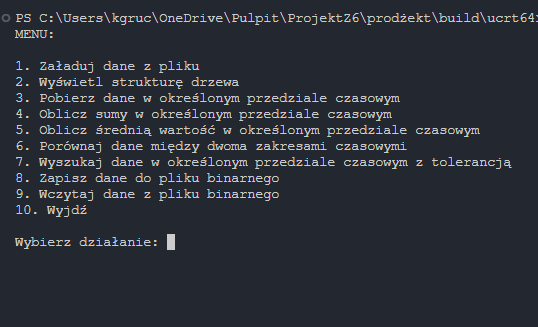
\includegraphics[width=0.8\linewidth]{img/1.png}
    \caption{Menu programu}
    \label{rys:rysunek1}
\end{figure}
\newpage
\noindent Teraz za pomocą 1 opcji użytkownik może wczytać do programu dane z pliku .csv, które można później poddać analizie, zostało to pokazane na rysunku nr. \ref{rys:rysunek2} (s. \pageref{rys:rysunek2}).
\\
\begin{figure}[h]
    \centering
    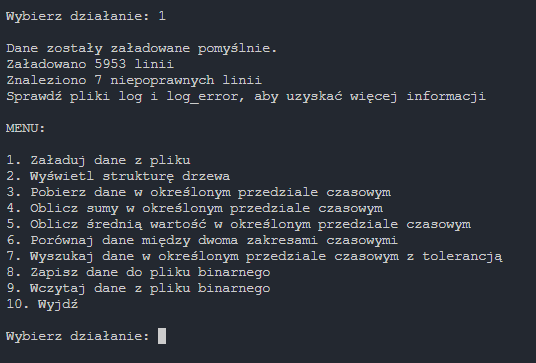
\includegraphics[width=0.8\linewidth]{img/2.png}
    \caption{Załadowanie pliku .csv}
    \label{rys:rysunek2}
\end{figure} \\
Jak widzimy na rysunku nr. \ref{rys:rysunek2} (s. \pageref{rys:rysunek2}) z pliku .csv zostało załadowane poprawnie 5953 linii, oraz znaleziono 7 niepoprawnych linii, aby uzyskać informacje na temat tego błędu, użytkownik może zobaczyć pliki z logami, które program generuje. Teraz możemy przejść do testu np. 3 opcji, wybieramy ją i wpisujemy ramy czasowe tak jak na rysunku nr. \ref{rys:rysunek3} (s. \pageref{rys:rysunek3})
\begin{figure}[h]
    \centering
    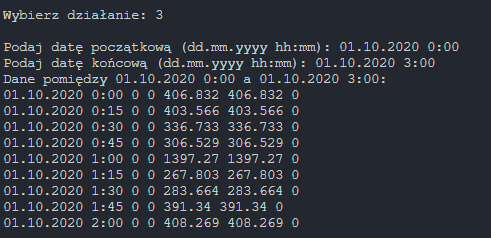
\includegraphics[width=0.8\linewidth]{img/4.png}
    \caption{Testowanie opcji}
    \label{rys:rysunek3}
\end{figure}
\newpage
\noindent Jak widzimy na rysunku nr. \ref{rys:rysunek3} (s. \pageref{rys:rysunek3}), dane zostały prawidłowo wypisane z pliku .csv zgodnie z wybranym przedziałem czasowym. Teraz możemy sobie zapisać nasze dane do plku binarnego, tak jak zostało to pokazane na rysunku nr.  \ref{rys:rysunek5} (s. \pageref{rys:rysunek5}).
\begin{figure}[h]
    \centering
    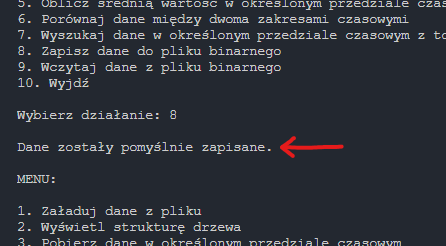
\includegraphics[width=0.8\linewidth]{img/5.png}
    \caption{Zapis do pliku binarnego}
    \label{rys:rysunek5}
\end{figure} \\
Możemy przetestować jeszcze 5 opcję która oblicza średnie wartości w określonym przedziale czasowym, działanie zostało przedstawione na rysunku nr. \ref{rys:rysunek6} (s. \pageref{rys:rysunek6}).
\begin{figure}[h]
    \centering
    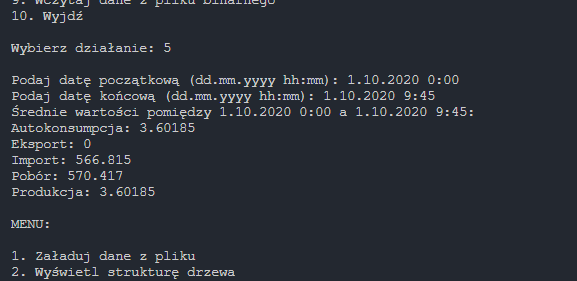
\includegraphics[width=0.8\linewidth]{img/6.png}
    \caption{Testowanie opcji programu}
    \label{rys:rysunek6}
\end{figure}
\newpage
\subsection{Testy programu}
W projekcie został przeprowadzony test za pomocą frameworka Google Test, który umożliwił dokładną weryfikację poprawności działania kluczowych modułów aplikacji. Na rysunku nr. \ref{rys:rysunek7} (s. \pageref{rys:rysunek7})  został przeprowadzony zrzut z wykonanych testów. 
\\ 
\begin{figure}[h]
    \centering
    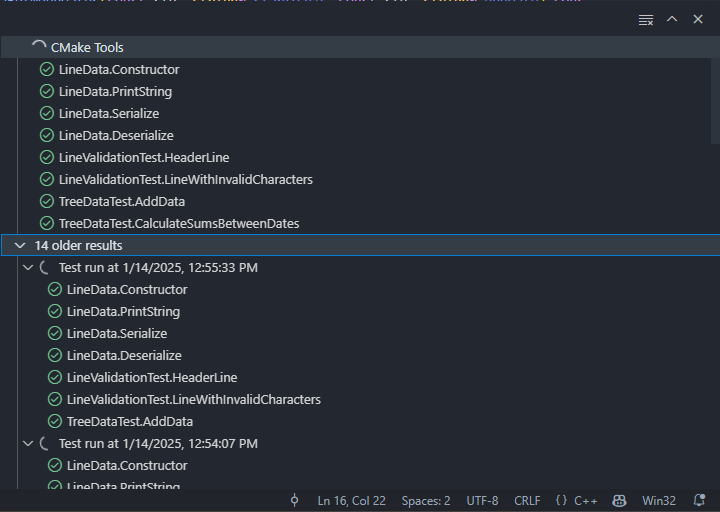
\includegraphics[width=0.8\linewidth]{img/test.png}
    \caption{Testy kodu za pomocą Google Test}
    \label{rys:rysunek7}
\end{figure} \\
\noindent Google Test został wybrany, ponieważ jest to narzędzie wydajne, elastyczne i dostosowane do wymagań projektu. Jego zastosowanie umożliwiło szybkie i dokładne przeprowadzenie testów jednostkowych, zwiększając niezawodność aplikacji. W projekcie do testowania można było jeszcze użyt takiego narzędzie jak Catch2 który jest bardzo łatwy w użyciu oraz ma intuicyjny system asercji i czytelne raport o wynikach testów, lecz jest mniej zaawansowany niż Google Test w przypadku bardziej złożonych scenariuszy, takich jak testy parametrów czy współpraca z dużymi projektami.
\newpage
\subsection{Pomoc AI w projekcie}
W projekcie został wykorzystany GitHub Copilot, który pomógł przy pisaniu różnych fragmentów kodu. AI szczególnie był pomocny przy:
\begin{itemize}
    \item \textbf{Generowanie szkieletu kodu} - Copilot był szczególnie pomocny w tworzeniu szkieletu kodu. Automatycznie proponował struktury funkcji, deklaracje klas oraz szablony kodu bazujące na nazwach funkcji i zmiennych. To znacznie przyspieszyło proces tworzenia początkowych wersji modułów, takich jak obsługa menu czy operacje na plikach.
    \item \textbf{Operacje na strukturach danych} - Podczas implementacji funkcji dla struktury drzewa (treeData.hpp), Copilot dobrze sugerował metody wyszukiwania, filtrowania i iteracji po węzłach. Przyspieszyło to implementację takich funkcji, jak obliczanie sum czy wyszukiwanie danych w przedziale czasowym.
    \item \textbf{Obsługa plików} - Przy implementacji funkcji wczytywania i zapisywania danych (CSV, binarne), Copilot pomógł w generowaniu kodu do operacji na plikach, takich jak otwieranie plików, odczytywanie danych w pętlach oraz zapisywanie ich w odpowiednich formatach. Umożliwiło to skrócenie czasu pracy nad tymi funkcjami.
\end{itemize}
Copilot nie był pomocny w kilku kwestiach:
\begin{itemize}
    \item \textbf{Specyficzne wymagania projektu} - Copilot często sugerował ogólne rozwiązania, które nie zawsze pasowały do wymagań projektu. Na przykład przy pracy z niestandardową strukturą drzewa (TreeData) lub specyficznym formatem danych w plikach CSV konieczne było ręczne dopracowywanie kodu. Podpowiedzi wymagały dostosowania do rzeczywistych potrzeb projektu.
    \item \textbf{Logika biznesowa i analizy danych} - Chociaż Copilot był pomocny w pisaniu szkieletu funkcji, nie zawsze trafnie rozumiał zaawansowane operacje, takie jak obliczanie średnich, porównywanie danych między zakresami czasowymi czy implementacja tolerancji w wyszukiwaniu. Te fragmenty wymagały manualnego dostosowania.
\end{itemize}

\newpage
\section{Wnioski}	%5
%Npisać wnioski końcowe z przeprowadzonego projektu, 
\nocite{www1}
\nocite{www2}
\nocite{www3}
\nocite{www4}
Realizacja projektu pozwoliła na stworzenie aplikacji umożliwiającej efektywne przetwarzanie i analizowanie danych energetycznych zapisanych w formacie CSV. Aplikacja spełnia założenia projektowe, zapewniając użytkownikom narzędzia do organizowania danych w hierarchiczną strukturę drzewa oraz przeprowadzania różnorodnych analiz. Podczas pracy nad projektem zidentyfikowano kluczowe wyzwania i rozwiązania, które miały istotny wpływ na jakość i funkcjonalność aplikacji.
\begin{enumerate}
    \item \textbf{Efektywność algorytmu i struktura danych} - Kluczowym elementem projektu było stworzenie wydajnego algorytmu organizowania danych w strukturę drzewa, co pozwala na szybki dostęp do informacji w różnych przedziałach czasowych. Zastosowanie struktury drzewa okazało się optymalnym rozwiązaniem, umożliwiającym łatwe zarządzanie danymi oraz przeprowadzanie operacji analitycznych. Dzięki temu użytkownicy mogą szybko uzyskać dostęp do wymaganych informacji oraz wykonywać obliczenia na danych w sposób efektywny.
    \item \textbf{Zarządzanie błędnymi danymi} - Projekt wymagał szczególnej uwagi w zakresie obsługi błędnych danych, takich jak puste linie, niekompletne rekordy czy powtarzające się wiersze. Zostały zaimplementowane mechanizmy walidacji, które umożliwiły odrzucanie błędnych danych i generowanie szczegółowych logów. Dzięki temu program jest odporny na błędy w danych wejściowych, co zapewnia jego niezawodność i stabilność w trakcie użytkowania.
    \item \textbf{Optymalizacja wydajności} - Przetwarzanie dużych zbiorów danych energetycznych wiąże się z koniecznością zoptymalizowania pamięci oraz algorytmów. W trakcie realizacji projektu zastosowano odpowiednie techniki optymalizacji, które pozwalają na efektywne przetwarzanie danych bez nadmiernego obciążania systemu. Zastosowanie języka C++ oraz narzędzi takich jak GitHub Copilot, pozwoliło na szybsze generowanie kodu oraz implementację algorytmów, co wpłynęło na skrócenie czasu rozwoju projektu.
\end{enumerate}
Projekt został zrealizowany zgodnie z założeniami i spełnia wymagania dotyczące efektywnego przetwarzania danych oraz analizy energii. Aplikacja zapewnia nie tylko odpowiednią funkcjonalność, ale również odporność na błędne dane wejściowe, wysoką wydajność oraz elastyczność w zarządzaniu danymi. Zastosowanie nowoczesnych narzędzi i technologii przyczyniło się do przyspieszenia procesu programowania oraz poprawy jakości aplikacji, co stanowi solidną podstawę do rozwoju projektu w przyszłości.



%%%%%%%%%%%%%%%%%%% koniec treść główna dokumentu %%%%%%%%%%%%%%%%%%%%%
\newpage
\addcontentsline{toc}{section}{Literatura}
\printbibliography

\newpage
\hypersetup{linkcolor=black}
\renewcommand{\cftparskip}{3pt}
\clearpage
\renewcommand{\cftloftitlefont}{\Large\bfseries\sffamily}
\listoffigures
\addcontentsline{toc}{section}{Spis rysunków}
\thispagestyle{fancy}

\newpage
\renewcommand{\cftlottitlefont}{\Large\bfseries\sffamily}
\def\listtablename{Spis tabel}
\addcontentsline{toc}{section}{Spis tabel}\listoftables
\thispagestyle{fancy}

\newpage
\renewcommand{\cftlottitlefont}{\Large\bfseries\sffamily}
\renewcommand\lstlistlistingname{Spis listingów}
\addcontentsline{toc}{section}{Spis listingów}\lstlistoflistings
\thispagestyle{fancy}



%lista rzeczy do zrobienia: wypisuje na koñcu dokumentu, patrz: pakiet todo.sty
\todos
%koniec listy rzeczy do zrobienia
\end{document}
